
\section{Руководство пользователя}

Для использования системы необходимо:
\begin{itemize}
\item{
 Чтобы она была установлена и настроена в соответствии с Руководством администратора.
}
\item{
 Веб-сервер доступен по сети из рабочей станции пользователя.
}
\item{
 На рабочей станции пользователя установлен один из веб-браузеров: 
Internet Explorer (версия >= 7), Google Chrome (версия >= 15.0), Firefox (версия >= 3.0).
}
\end{itemize}


\subsection*{Начало работы}

В начале работы пользователь вводит в адресную строку браузера URL-адрес веб-сервера.
В случае, если сессия не была инициализирована, будет открыта страница входа.

Предполагается, что пользователь знаком с предметной областью IPTV услуг.

\begin{figure}[!ht]
\begin{center}
\hspace*{-1cm} 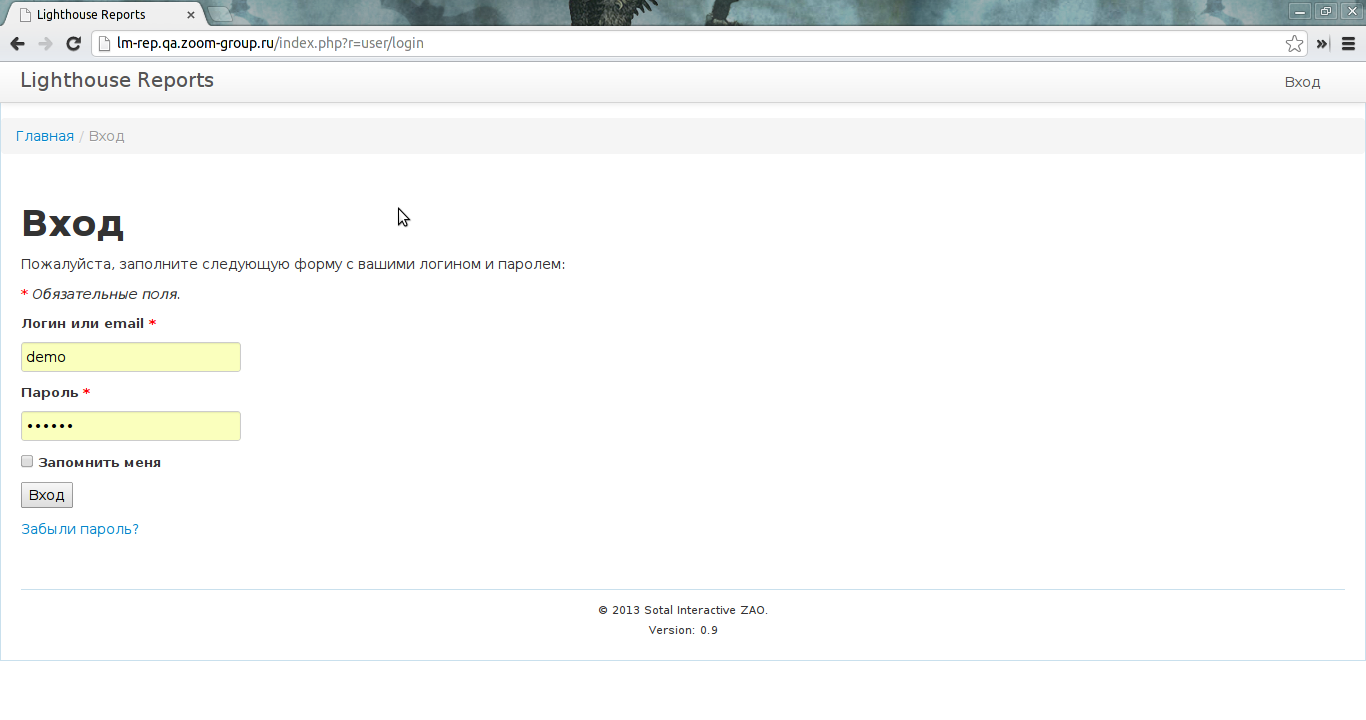
\includegraphics[scale=0.35, trim=0mm 0mm 0mm 10mm, clip]{../resources/screens/login.png}
\end{center}
\end{figure}

\begin{figure}[!ht]
\begin{center}
\hspace*{-1cm} 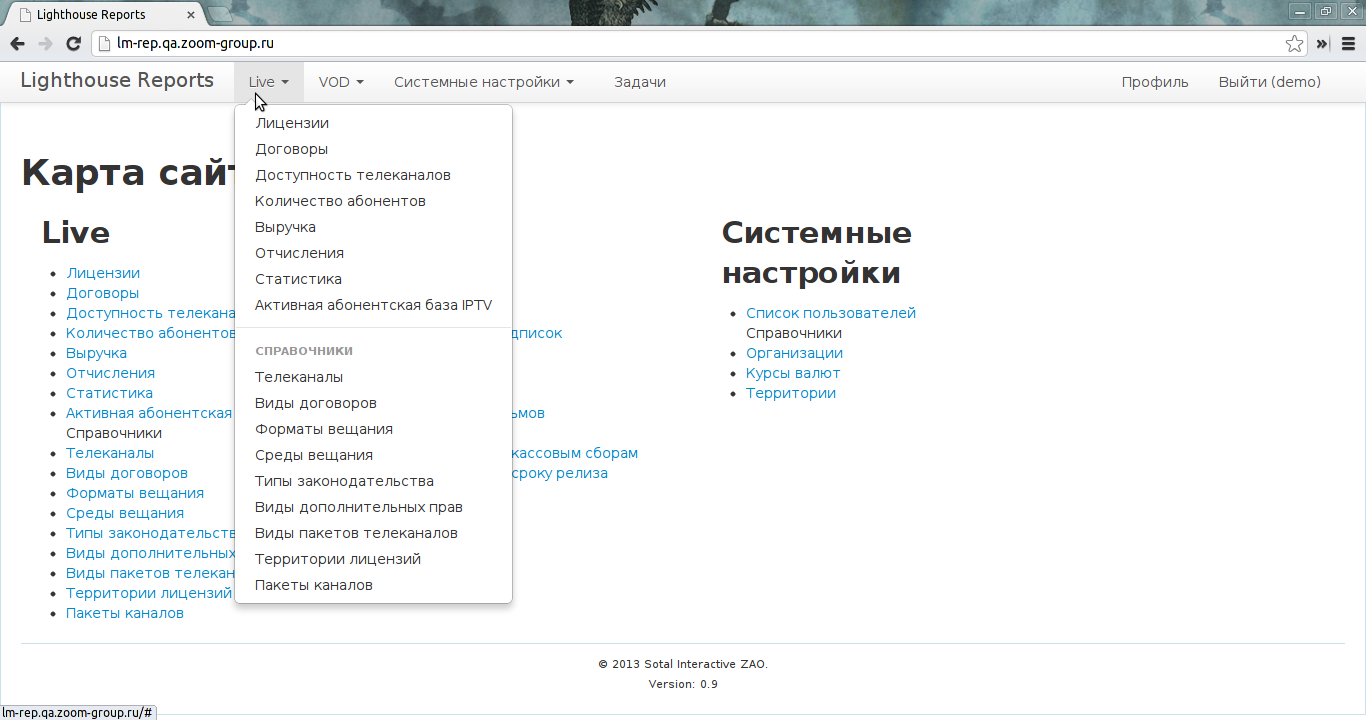
\includegraphics[scale=0.28, trim=0mm 0mm 0mm 10mm, clip]{../resources/screens/map.png}
\end{center}
\end{figure}

\vspace*{-1cm} 

После ввода правильных аутентификационных реквизитов, открывается Карта сайта --- раздел системы, в котором
выведены все доступные пользователю разделы системы. Кроме карты сайта, доступные разделы
также расположены в Главном меню.

Приложение состоит из трех разделов: Live, VOD и Системные настройки.

\subsection*{Работа с данными}

Большая часть ссылок из подразделов предоставляют интерфейс для поиска/редактирования данных
определенного вида (примеры на рисунках).

\begin{figure}[!ht]
\begin{center}
\hspace*{-1cm} 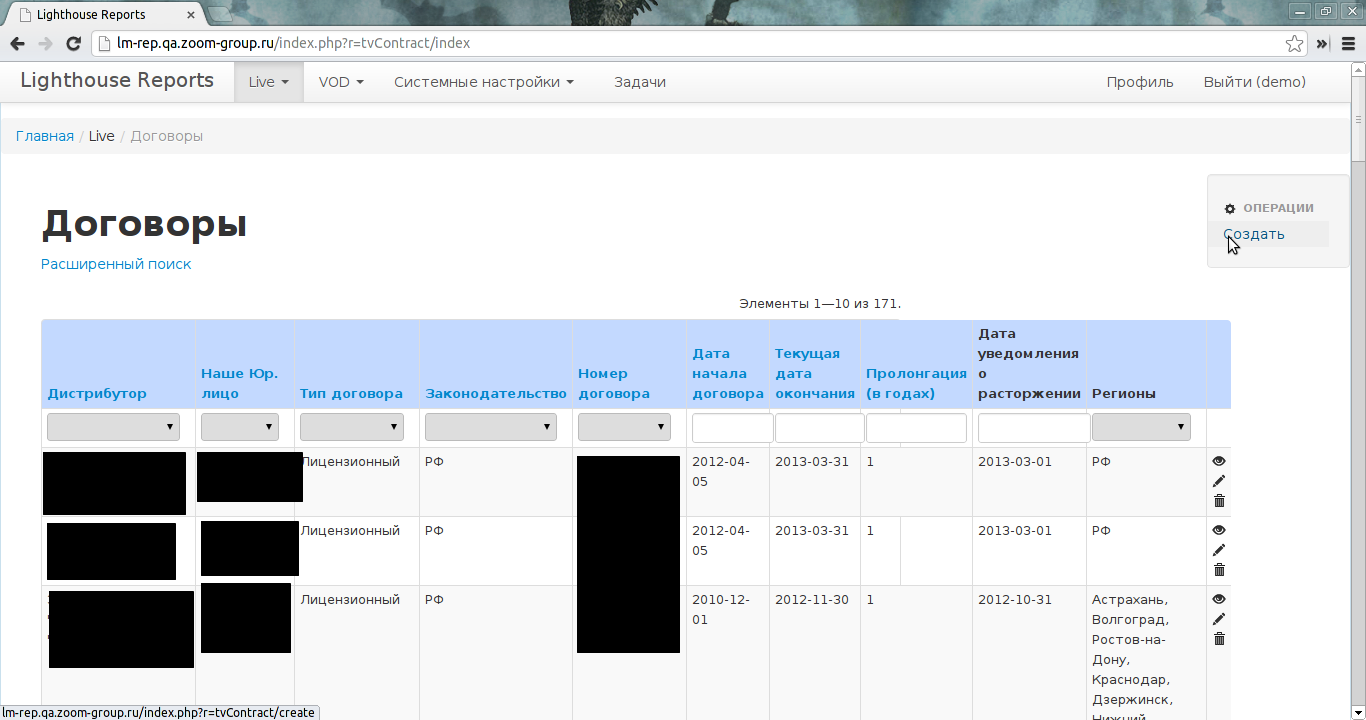
\includegraphics[scale=0.35, trim=0mm 0mm 0mm 10mm, clip]{../resources/screens/contracts.png}
\caption{Главная страница подраздела Live -> Договоры}
\end{center}
\end{figure}

\begin{figure}[!ht]
\begin{center}
\hspace*{-1cm} 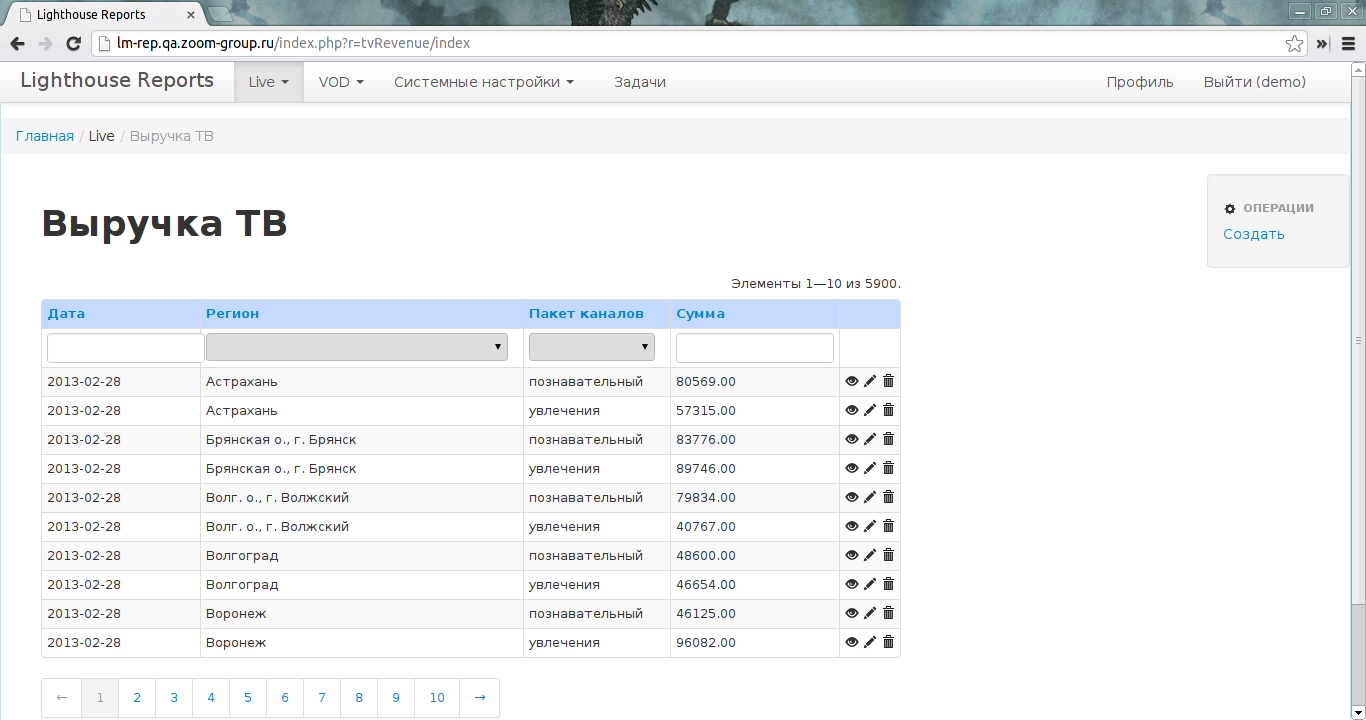
\includegraphics[scale=0.35, trim=0mm 0mm 0mm 10mm, clip]{../resources/screens/tv_revenue.png}
\caption{Главная страница подраздела Live -> Выручка ТВ}
\end{center}
\end{figure}

\begin{figure}[!ht]
\begin{center}
\hspace*{-1cm} 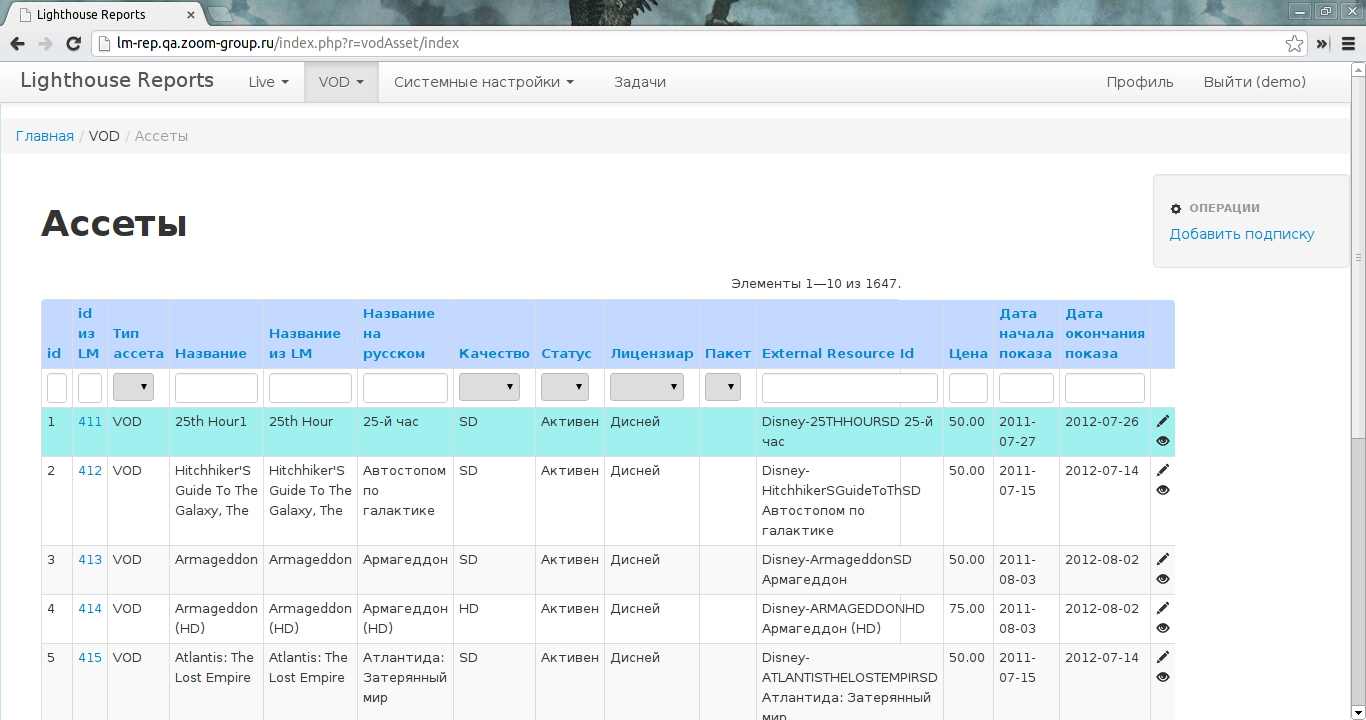
\includegraphics[scale=0.35, trim=0mm 0mm 0mm 10mm, clip]{../resources/screens/assets.png}
\caption{Главная страница подраздела VOD -> Ассеты}
\end{center}
\end{figure}

Находясь на главной странице такого интерфейса, пользователю доступен список объектов в виде таблицы.

Для фильтрации по значению нужно ввести необходимо ввести ключевое слово над соответствующим столбцом,
после чего произойдет обновление содержимого.

Для указания поля сортировки необходимо кликнуть по тексту заголовка соответсвующего столбца. 
Повторные нажатия изменят порядок сортировки или вернут сортировку по умолчанию.

В большинстве подобных интерфейсов присутствуют дополнительные операции, такие как например добавление объекта
(на рисунках в правом верхнем углу).

Для просмотра отдельного объекта нужно кликнуть по иконке с глазом в соответствующей строке.

Для редактирования объекта необходимо нажать на иконку с изображением карандаша, после этого браузер пользователя
перенаправляется на страницу редактирования.

\begin{figure}[!ht]
\begin{center}
\hspace*{-1cm} 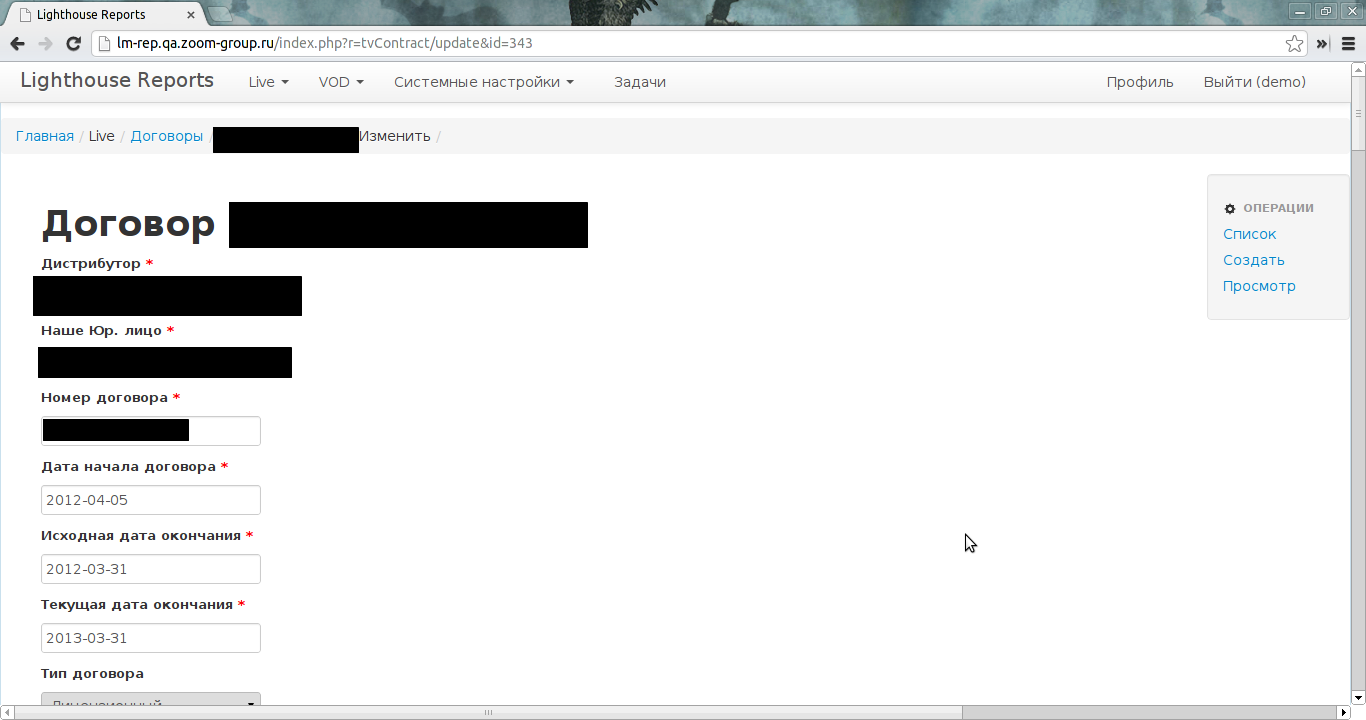
\includegraphics[scale=0.35, trim=0mm 0mm 120mm 10mm, clip]{../resources/screens/contract_edit.png}
\caption{Страница редактирования подраздела Live -> Договоры}
\end{center}
\end{figure}

\begin{figure}[!ht]
\begin{center}
\hspace*{-1cm} 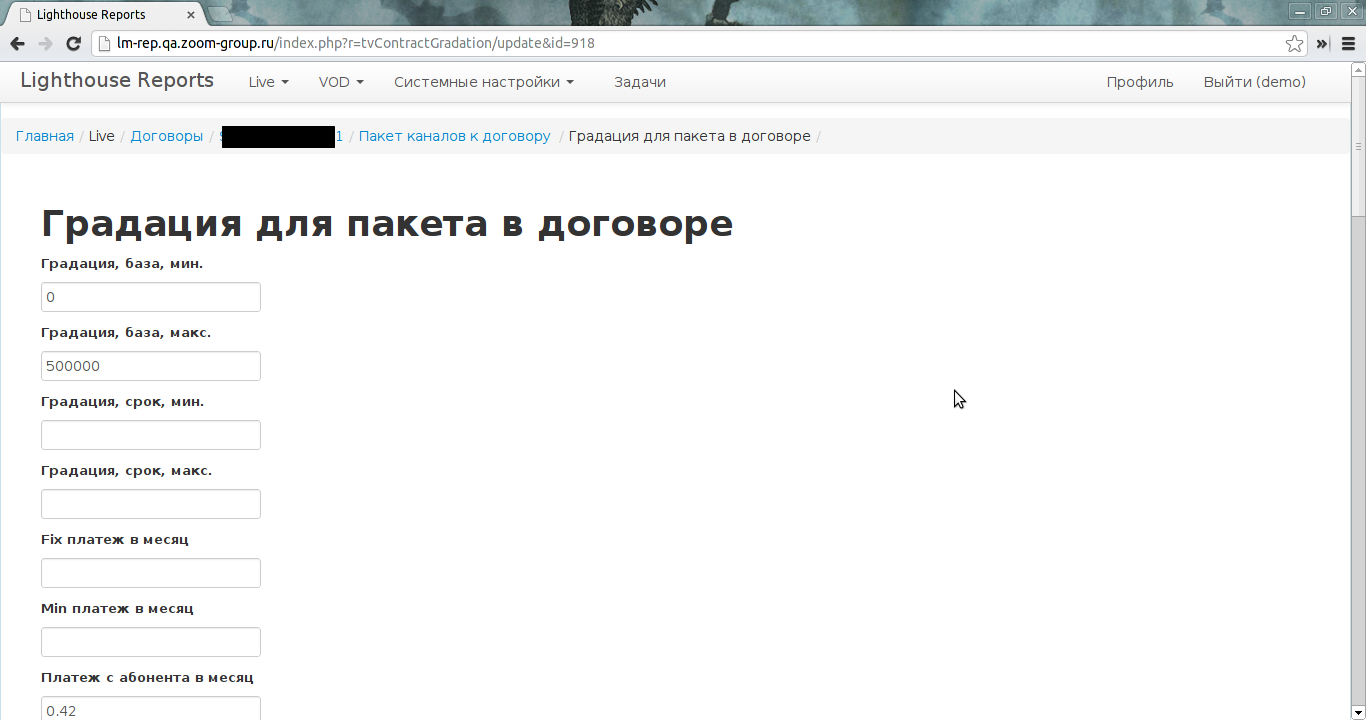
\includegraphics[scale=0.35, trim=0mm 0mm 120mm 10mm, clip]{../resources/screens/contract_gradation.png}
\caption{Страница редактирования градации по договору Live}
\end{center}
\end{figure}

На страницах с формами для редактирования/добавления объектов пользователь может заполнить
необходимые поля и сохранить объект, нажав кнопку "Сохранить" в нижней части страницы.

\begin{figure}[!ht]
\begin{center}
\hspace*{-1cm} 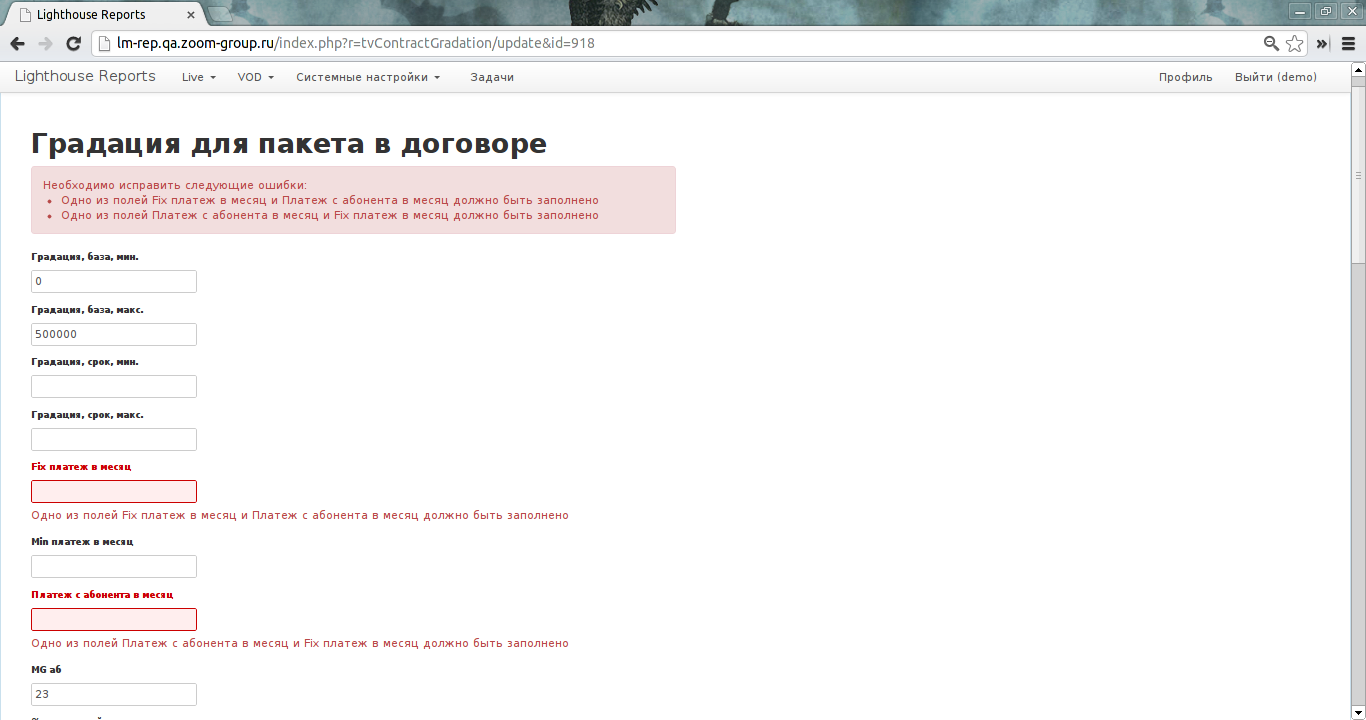
\includegraphics[scale=0.35, trim=0mm 0mm 120mm 10mm, clip]{../resources/screens/contract_gradation_error.png}
\caption{Страница редактирования градации по договору Live. Ошибка}
\end{center}
\end{figure}

В случае если данные формы были заполнены некорректно, объекты не сохраняются,
пользователю выводится уведомление в верхней части страницы. 
Кроме того поля с ошибочными значениями подсвечиваются красным цветом.

\subsection*{Задачи}

\begin{figure}[!ht]
\begin{center}
\hspace*{-1cm} 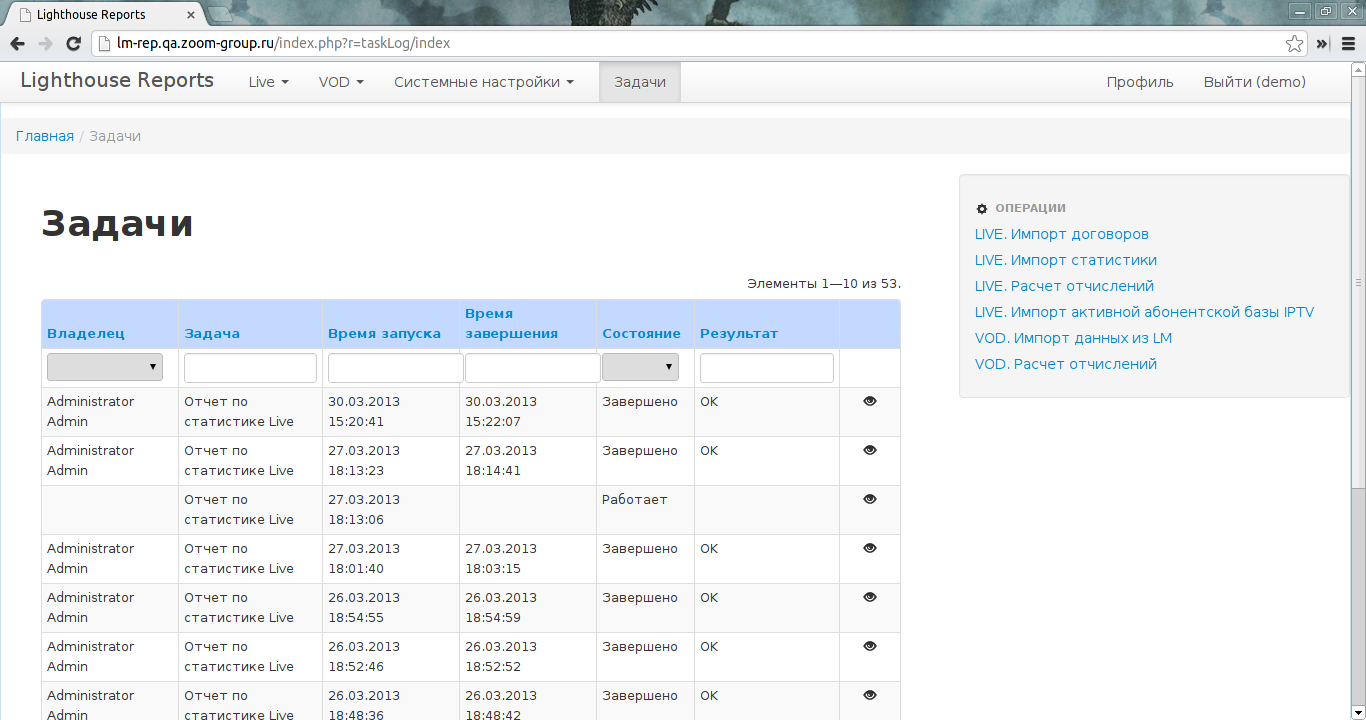
\includegraphics[scale=0.35, trim=0mm 0mm 0mm 10mm, clip]{../resources/screens/tasks.png}
\caption{Раздел задачи}
\end{center}
\end{figure}

В разделе "Задачи" пользователь может отслеживать статус запущенных им фоновых задач
и инициировать запуск новых.

Для просмотра результата завершенной задачи нужно кликнуть по пиктограмме с изображением глаза,
в случае, если результатом работы задачи был файл, он доступен для скачивания.

Для запуска доступны следующие задачи:
\begin{itemize}
\item{
  Импорт договоров по Live из файла в формате Microsoft Excel
}
\item{
  Импорт статистических данных по Live из файла в формате XML
}
\item{
  Расчет отчислений по Live
}
\item{
  Импорт активной абонентской базы из файла в формате Microsoft Excel
}
\item{
  Импорт данных для VOD 
}
\item{
  Расчет отчислений по VOD
}
\end{itemize}

\begin{figure}[!ht]
\begin{center}
\hspace*{-1cm} 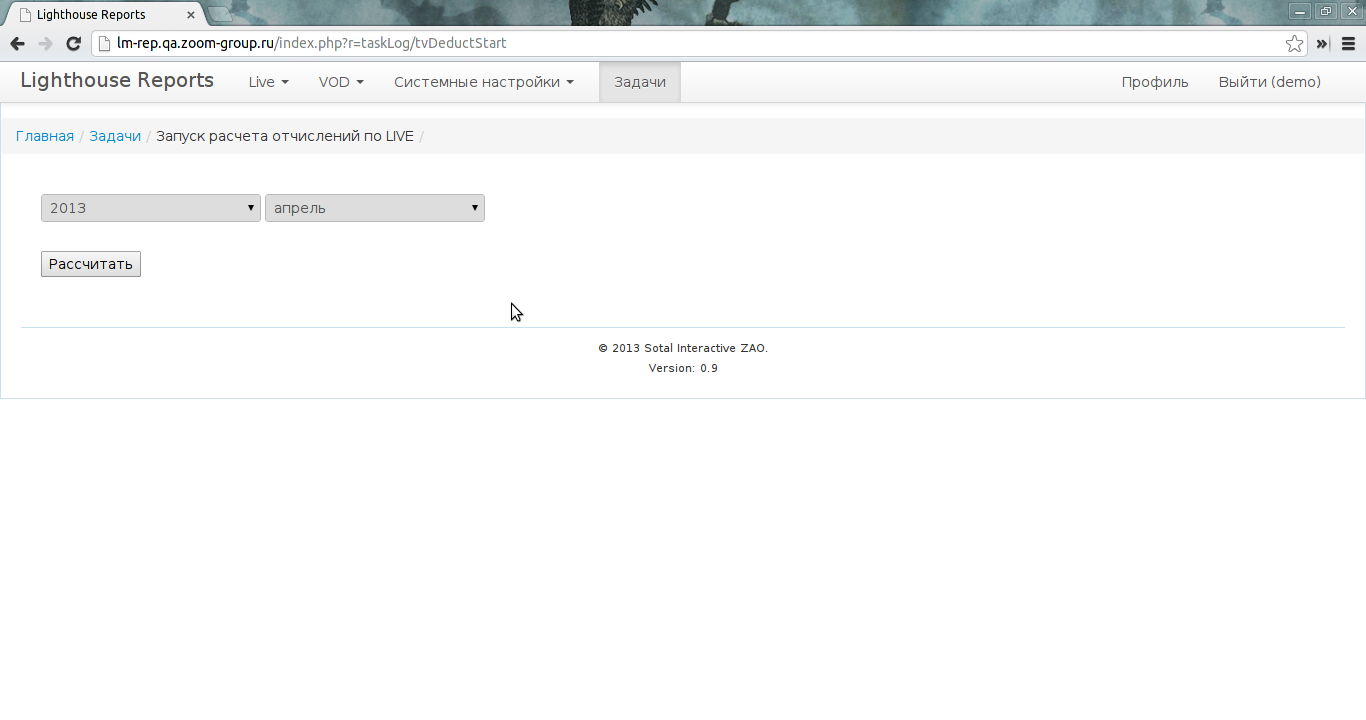
\includegraphics[scale=0.35, trim=0mm 70mm 250mm 10mm, clip]{../resources/screens/deduct_start.png}
\caption{Интерфейс запуска для расчета отчислений по Live}
\end{center}
\end{figure}

\subsection*{Генерация отчетов}
Для работы со статистическими отчетами по Live или VOD необходимы выбрать
в соответствующем разделе меню пункт ``Статистика'', после чего пользователю
становится доступна форма параметров отчета.

Выбранные в форме параметры сохраняются для данного пользователя и могут быть
доступны в рамках последующих сессий использования.

\begin{figure}[!ht]
\begin{center}
\hspace*{-1cm} 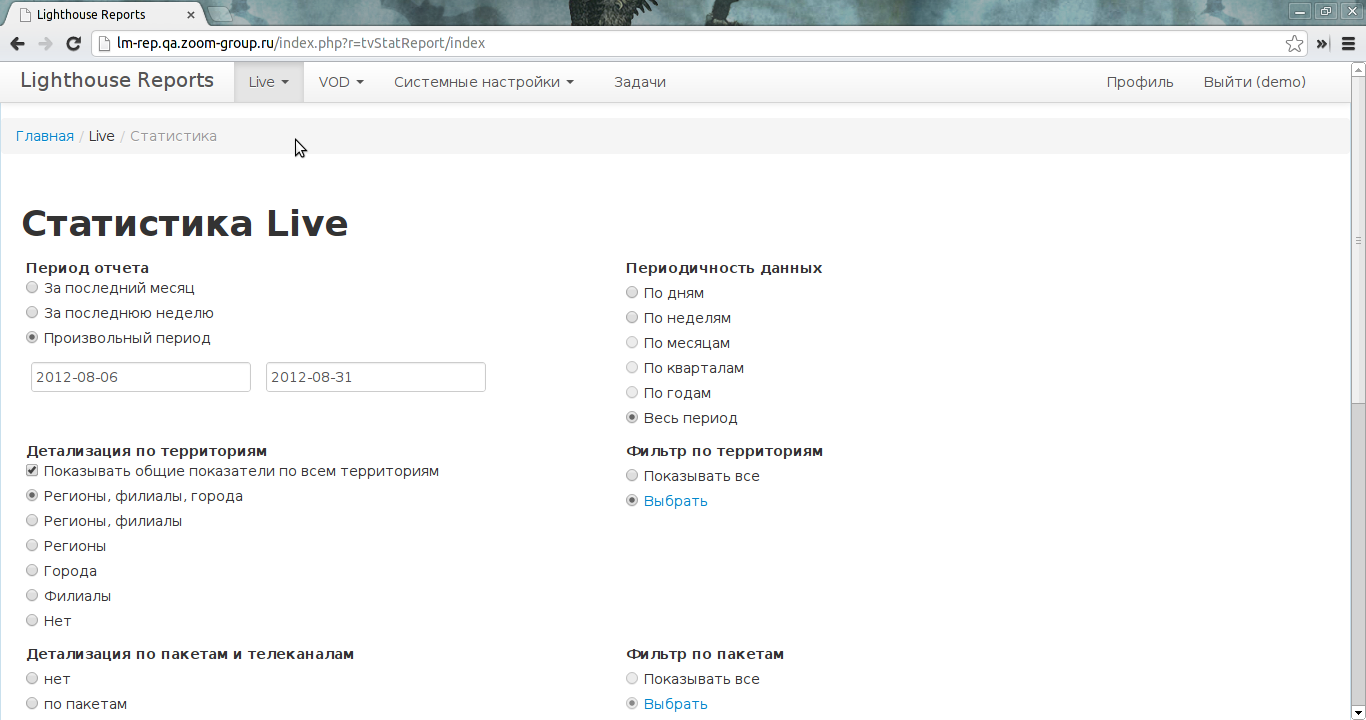
\includegraphics[scale=0.35, trim=0mm 0mm 180mm 10mm, clip]{../resources/screens/live_stat.png}
\caption{Страница Live / Статистика}
\end{center}
\end{figure}

\begin{figure}[!ht]
\begin{center}
\hspace*{-1cm} 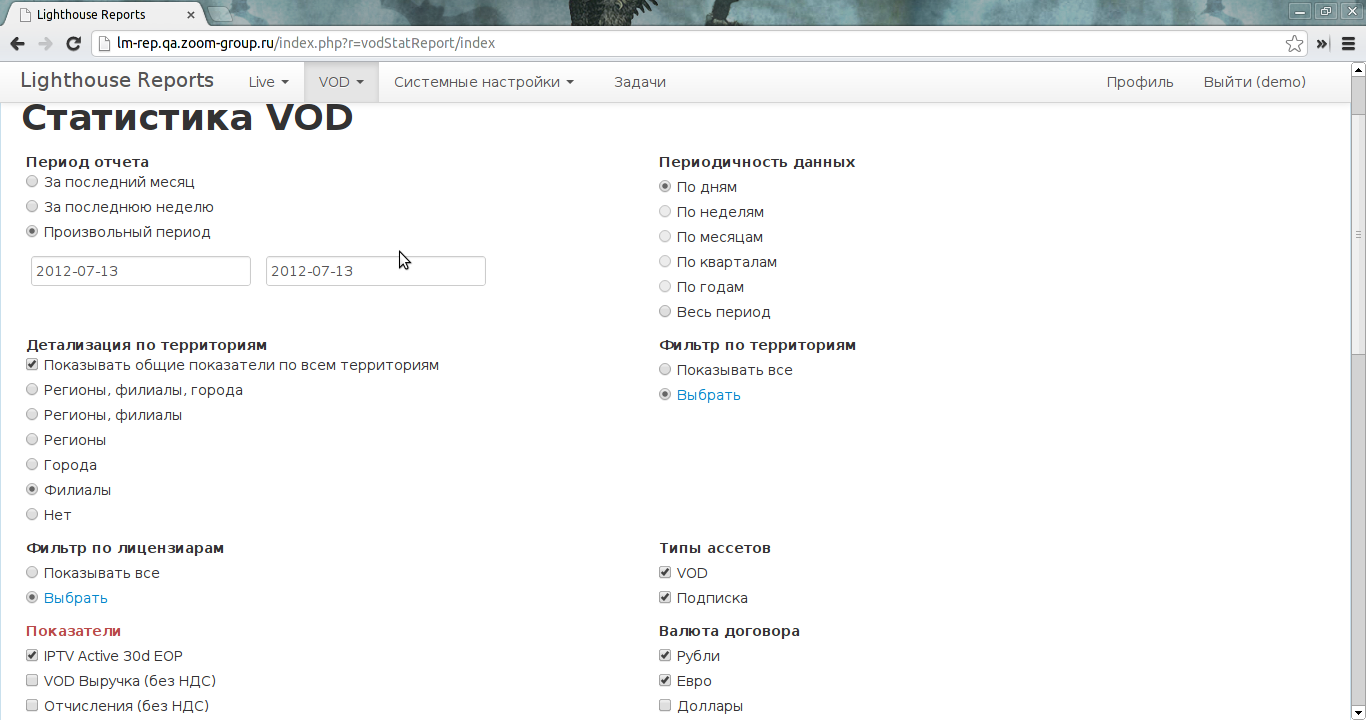
\includegraphics[scale=0.35, trim=0mm 0mm 180mm 10mm, clip]{../resources/screens/vod_stat.png}
\caption{Страница VOD / Статистика}
\end{center}
\end{figure}

\paragraph{Период}
Пользователь может выбрать период отчета из фиксированных вариантов: ``За прошлую неделю''/``За прошлый год''
или указать произвольный интервал дат в полях под надписью ``Произвольный период''.
При нажатии на поле с датой становится доступен вспомогательный элемент с календарем, где может быть
выбран определенный день месяца.

В разделе ``Периодичность данных'' определяется, каким образом выбранный период будет разбиваться на подинтервалы,
для каждого из которых будут вычислены значения показателей.
Варианты разбиения указаны на рисунке и комментариях не нуждаются.

\paragraph{Территории}
Для определения детализации по территориям необходимо выбрать один из пунктов
переключателя в соответствующем разделе страницы формы.
В случае, если отмечен флажок ``Показывать общие показатели по всем территориям'',
то независимо от типа детализации, будут вычислены значения суммарно по всем
территориям (РФ). 

``Фильтр по территориям'' определяет множество регионов, которые будут 
выведены в отчете. При выборе пункта ``Выбрать'' во всплывающем окне будет выведено дерево
территорий в соответствии с текущим типом детализации, где для каждого 
региона, который необходимо вывести должен быть установлен флажок.
В верхней части всплывающего окна доступны кнопки ``Выбрать все'', ``Очистить выбор''.

\begin{figure}[!ht]
\begin{center}
\hspace*{-1cm} 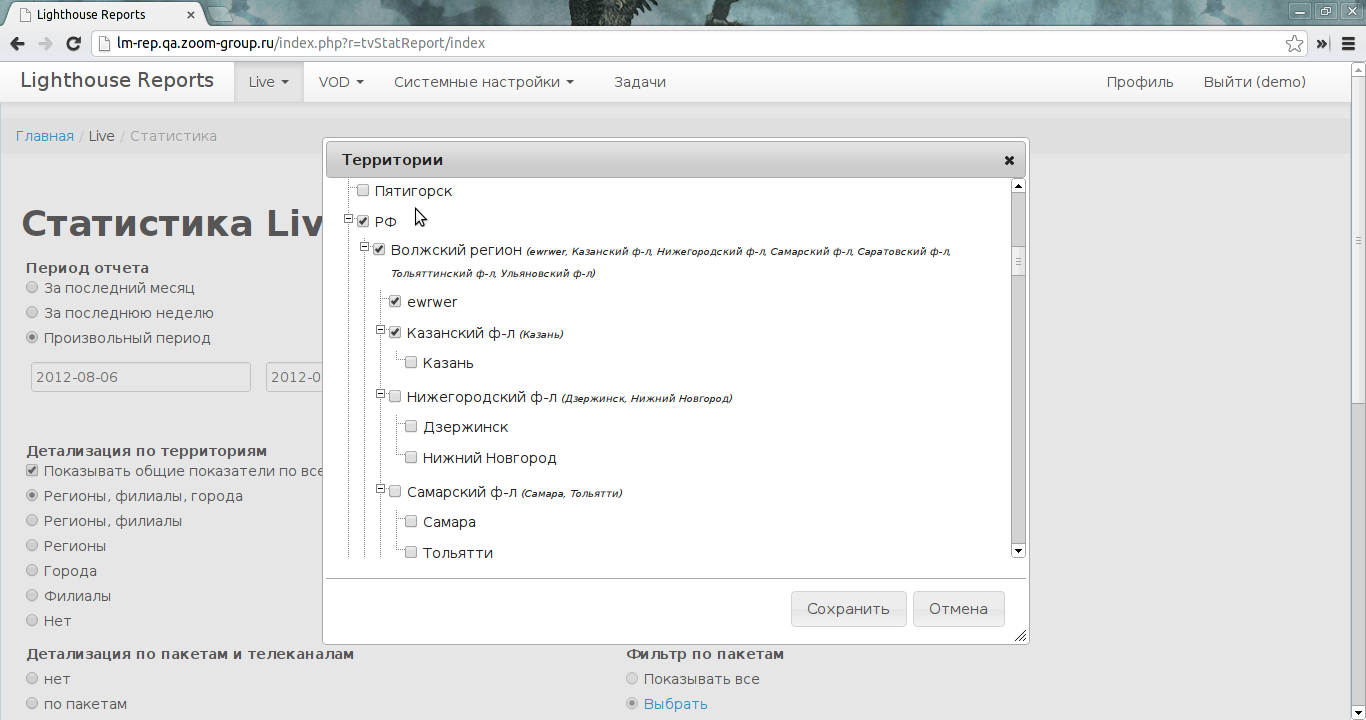
\includegraphics[scale=0.35, trim=0mm 0mm 100mm 10mm, clip]{../resources/screens/live_stat_regions.png}
\caption{Страница Live / Статистика. Фильтр регионов}
\end{center}
\end{figure}

\paragraph{Пакеты и телеканалы}
Функциональность по выбору детализации по пакетам и телеканалам в целом аналогична 
выбору детализации по территориям. Сначала пользователь выбирает один из уровней детализации:
\begin{itemize}
\item{
  Без детализации
}
\item{
  По пакетам
}
\item{
  По телеканалам
}
\item{
  По пакетам, затем по телеканалам
}
\item{
  По телеканалам, затем по пакетам
}
\end{itemize}

После этого в соответствующих фильтрах выбираются пакеты и телеканалы, 
данные по которым должны быть включены в отчет.

\paragraph{Выбор показателей}
В нижней части формы расположен раздел для выбора показателей,
необходимых для вычислений в рамках текущего отчета.
Выбранные показатели отмечаются флажками.

\begin{figure}[!ht]
\begin{center}
\hspace*{-1cm} 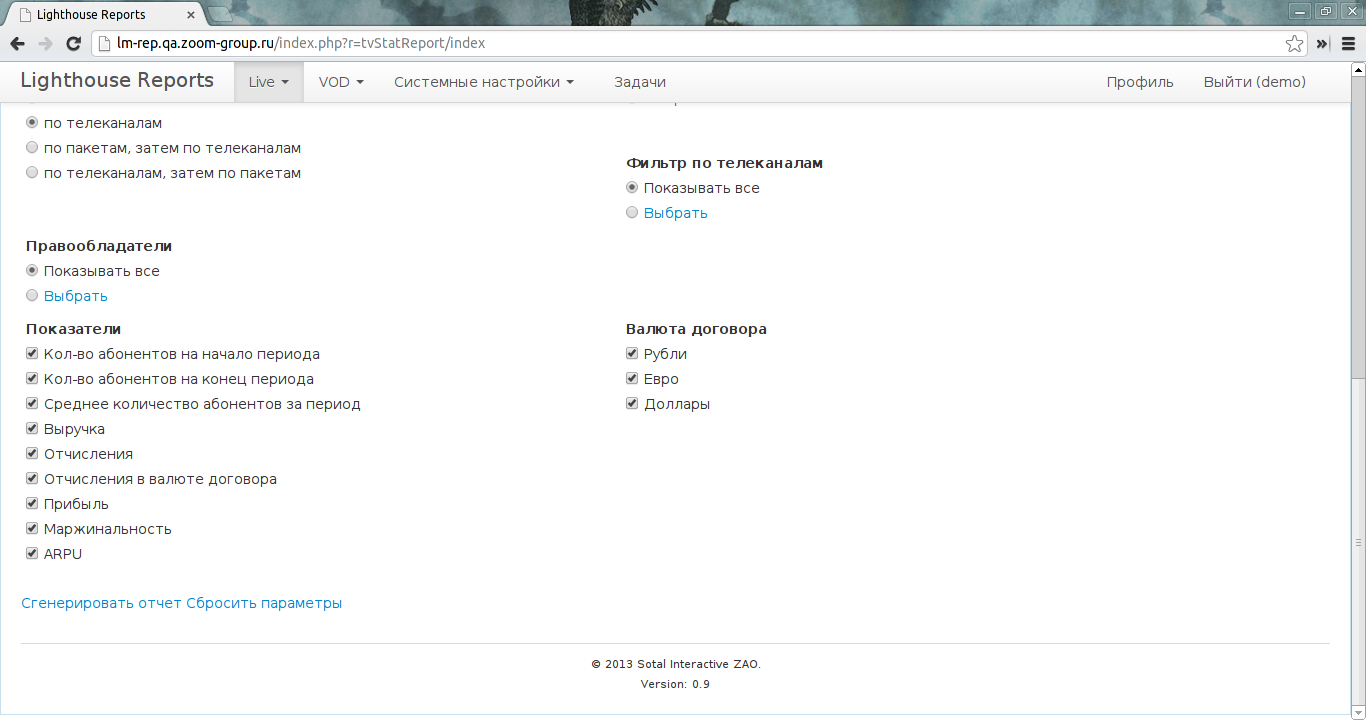
\includegraphics[scale=0.35, trim=0mm 0mm 100mm 10mm, clip]{../resources/screens/live_stat_indicators.png}
\caption{Страница Live / Статистика. Выбор показателей}
\end{center}
\end{figure}

\paragraph{Создание отчета}
После установки параметров пользователь может запустить процесс
генерации отчета, кликнув по кнопке "Сгенерировать отчет".
После этого браузер пользователя перенаправляется на страницу ожидания,
где будет выведен статус выполнения задачи. После окончания процесса
будет инициализировано скачивание файла с отчетом в формате Microsoft Excel.

\begin{figure}[!ht]
\begin{center}
\hspace*{-1cm} 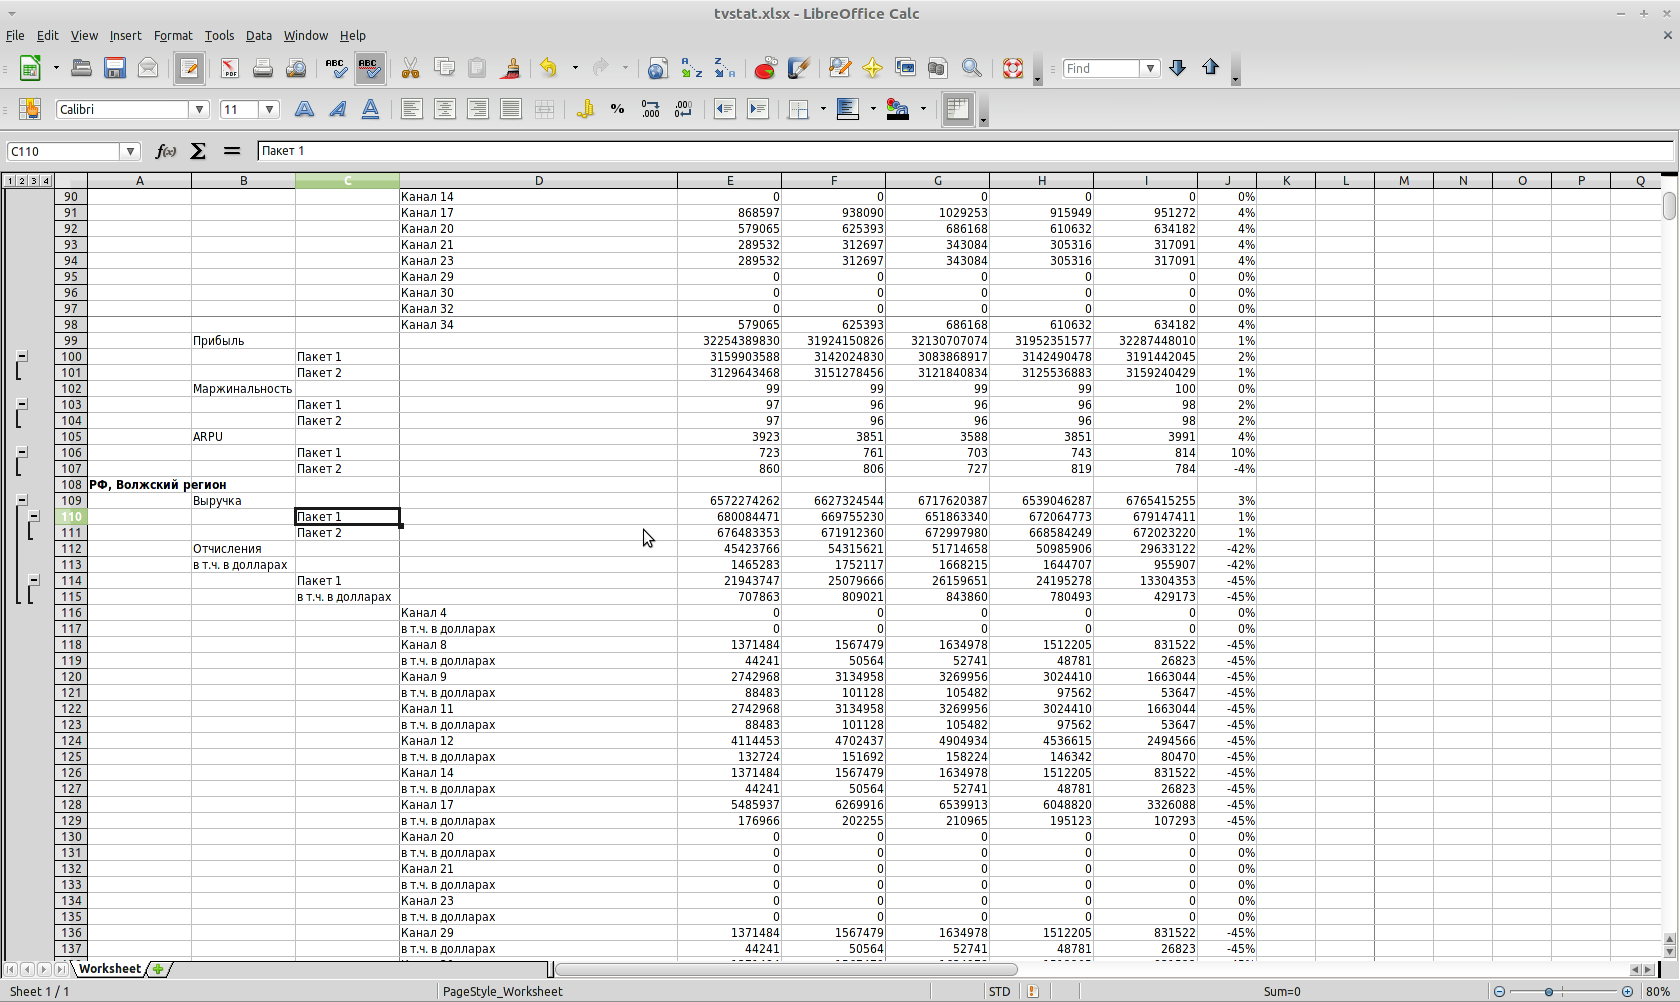
\includegraphics[scale=0.35, trim=0mm 100mm 150mm 50mm, clip]{../resources/report1.png}
\caption{Содержимое файла отчета}
\end{center}
\end{figure}

\paragraph{Структура отчетов}
Файл отчета представляет собой таблицу Excel, первые
столбцы описывают уровень детализации строки. В последующих столбцах
расположены значения показателей для каждого подинтервала, заключающий столбец
содержит значение End Of Percent показателя.

Каждый уровень детализации может быть скрыт с помощью группировки вложенности
таблиц путем нажатия на пиктограммы ``-''/``+''.

В случае, если при определении параметров отчета на форме, были выбраны валюты,
то строки с показателями по Отчислениям будут дублироваться строками значений
в выбранных валютах.

\subsection*{Рекомендации по созданию отчета}
При заполнении формы параметров необходимо учитывать размер получаемого файла с отчетом,
так например при открытии файла с количеством строк, превышающим 10000, наблюдается
значительное замедление работы редактора Microsoft Excel.

Таким образом следует как можно точнее определять цель, преследуемую при запросе
отчета, и в соответствии с этим выбирать только нужные уровни детализации, территории,
периоды и другие фильтры.

